\chapter{Mapping of IEEE LTSA Framework in Service Oriented Architecture (SOA) for further Improvement}
 \blindtext, as was
the case with the components \cite{lan}.
\begin{figure}[h!]
 \centering
 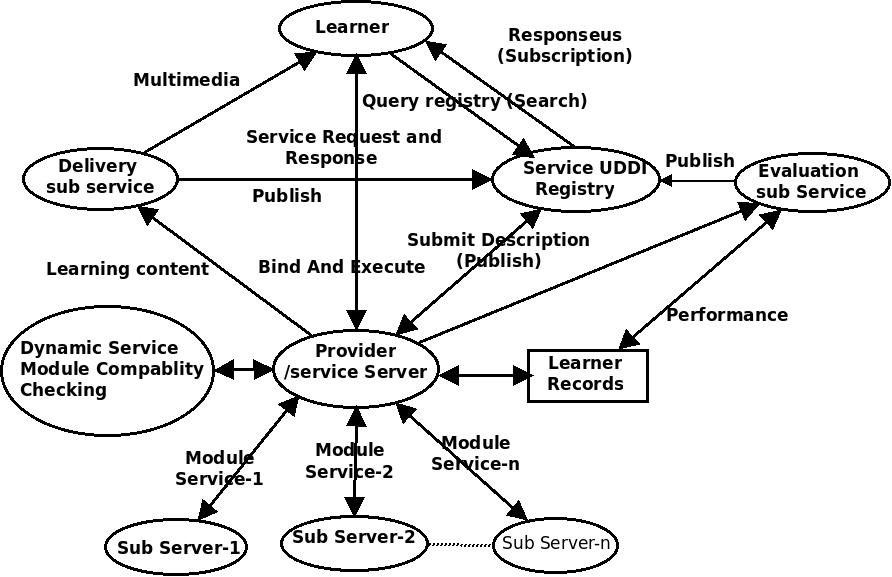
\includegraphics[scale=.5]{s0ajournal.jpeg}
 % s0ajournal.jpeg: 892x577 pixel, 72dpi, 31.47x20.36 cm, bb=0 0 892 577
 \caption{IEEE LTSA in SOA environment}
\end{figure}

    \blindtext.\\

   The proposed extended model of IEEE LTSA makes use of SOA architecture
(Figure. 5). \blindtext
\section{Capabilities of the proposed Service Oriented Architecture based IEEE LTSA Model}
The analysis of the model as presented in Figure. 5 brings out the following inherent
capabilities in the proposed extended model of IEEE LTSA:
\begin{itemize}
 \item \textit{Reusability}- SOA based IEEE LTSA model provide reuseability of learning services because they are loosly coupled. A new composition of different services
is possible by permutation, combination of the services and feasibility of their composition.
\item \textit{Interoperability}- SOA based model stresses interoperability, the ability of
systems using different platforms and languages to communicate with each other.
Each learning service provides an interface that can be invoked through a connector
type. An interoperable connector consists of a protocol and a data format, that
each of the potential user of the service understands. Interoperability is achieved
by supporting the protocol and data formats of the service’s current and potential
users including learners.
\item \textit{Loose Coupling}- Coupling refers to the number of dependencies between
modules. There are two types of coupling: loose and tight. Loosely coupled modules have a few well-known dependencies. Tightly coupled modules have many well
known as well as unknown dependencies. Every software architecture strives to
achieve loose coupling between modules. SOA promotes loose coupling between
service consumers and service providers. A few well-known dependencies between
consumers and providers may even be restored to become independent under imposed conditions. This may promote the composed components
 or modules to perform efficiently without infection of other components and modules. The conditional loose coupling allows to run 
the composed service faster in a stand alone
manner.
\item \textit{Flexibility}-The loosely-coupled, document-based, asynchronous nature of
services in an SOA allows e-learning applications to be flexible. With changing
requirements, the adaptability comes faster.
\item \textit{Capability of providing composite e-learning services}- The proposed framework is having the capability like scaling, 
suitability of high performance, customerization and coupling/decoupling of services depending upon the circumstances.

\end{itemize}

